\chapter{Assistência estudantil}
\DoPToC
\section{Bibliotecas}
    A UFBA dispõe de 22 (vinte e duas) bibliotecas que oferecem empréstimos gratuitos de material bibliográfico aos estudantes da UFBA.
    \begin{wrapfigure}{R}{0.3\textwidth}
            \centering
            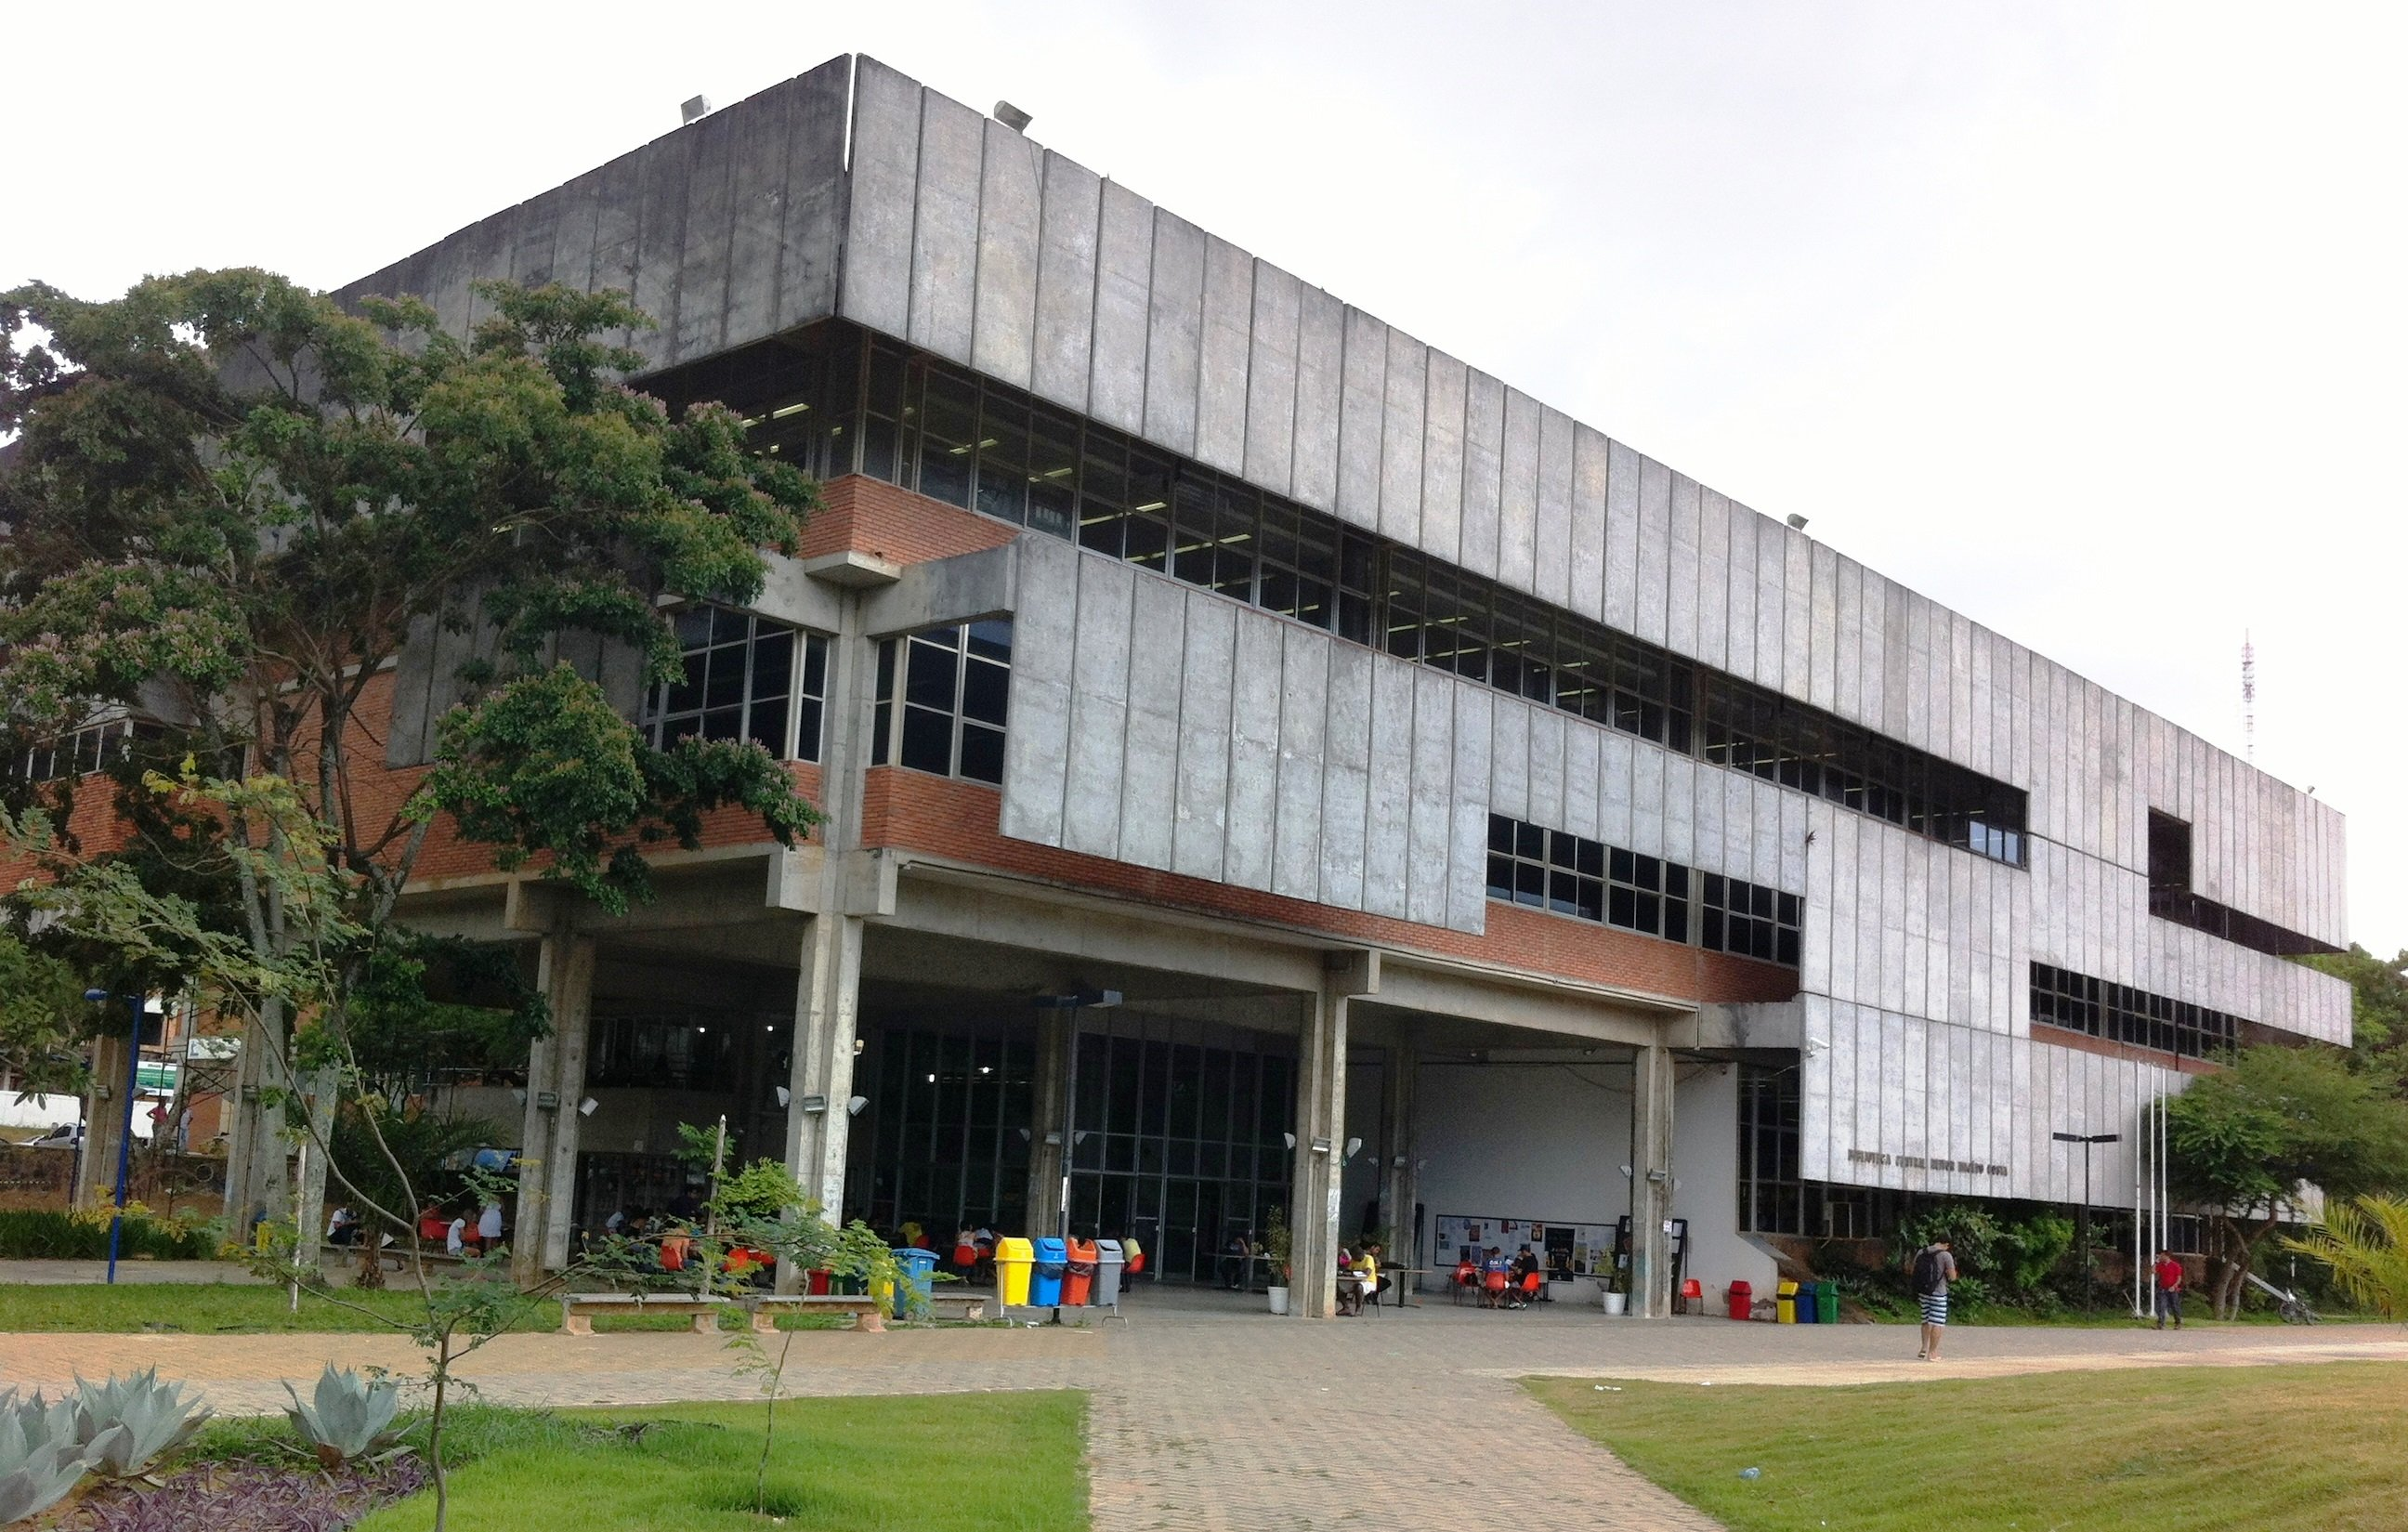
\includegraphics[width=0.29\textwidth]{biblioteca}
        \end{wrapfigure}
    \subsubsection{Biblioteca Universitária Reitor Macedo Costa}
        \begin{itemize}
            \item Abriga acervo do Instituto de Letras, Faculdade de Comunicação, Instituto de Humanidades, Artes e Ciências, Instituto de Biologia, Faculdade de Farmácia, Escola de Medicina Veterinária, Escola de Dança, além de coleções especiais.
            \item Horário de funcionamento: segunda a sexta-feira, das 7:30h às 21:00h e sábado e domingo das 8:00h às 16:00h.
            \item Endereço: Rua Barão de Jeremoabo, s/n, Campus Universitário de Ondina, 40170-290 - Salvador
        \end{itemize}
        
        \newpage
\begin{wrapfigure}{R}{0.3\textwidth}
    \centering
    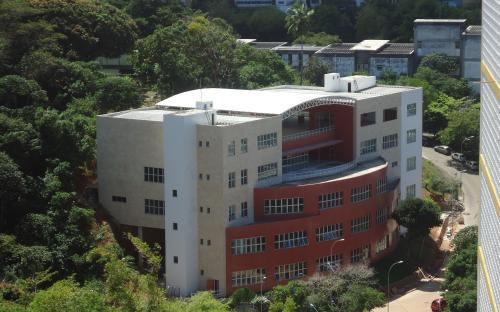
\includegraphics[width=0.29\textwidth]{biblioteca20_exatas}
\end{wrapfigure}
    \subsubsection{Biblioteca Universitária de Exatas Omar Catunda}
        \begin{itemize}
            \item Abriga acervo acervo da área das ciências exatas – Matemática, Estatística, Ciência da Computação, Física e Química - e também o acervo de Geociências.
            \item Horário de funcionamento: segunda a sexta-feira, das 7:30h às 21:00h.
            \item Endereço: Rua Barão de Jeremoabo, s/n, 40170-290 - Salvador.
        \end{itemize}
    \begin{wrapfigure}{R}{0.3\textwidth}
            \centering
            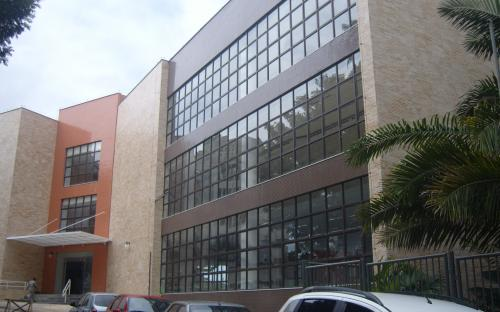
\includegraphics[width=0.29\textwidth]{biblioteca2_bus}
    \end{wrapfigure}
    \subsubsection{Biblioteca Universitária de Saúde Prof. Álvaro Rubim de Pinho}
        \begin{itemize}
            \item Abriga acervo da Escola de Enfermagem, Escola de Nutrição, Faculdade de Medicina, Faculdade de Odontologia, Instituto de Ciências da Saúde, Instituto de Saúde Coletiva e do Hospital Universitário Prof. Edgard Santos.
            \item Horário de funcionamento: segunda a sexta-feira, das 7:30h às 21:00h e sábado das 8:00h às 16:00h.
            \item Endereço: Rua Basílio da Gama, s/n, Canela, 40110-907 - Salvador
        \end{itemize}
    \begin{wrapfigure}{R}{0.3\textwidth}
            \centering
            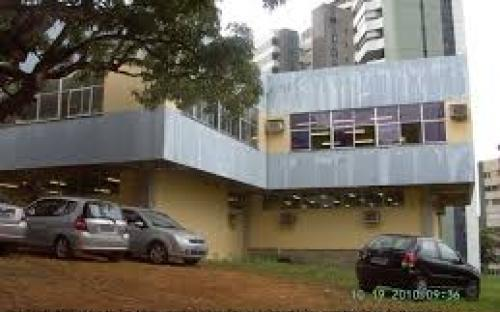
\includegraphics[width=0.29\textwidth]{biblioteca3_fch}
    \end{wrapfigure}
    \subsubsection{Biblioteca Universitária Isaías Alves}
        \begin{itemize}
            \item Abriga acervo da Faculdade de Filosofia e Ciências Humanas e do Instituto de Psicologia.
            \item Horário de funcionamento: segunda a sexta-feira, das 8:00h às 17:00h.
            \item Endereço: Estrada de São Lázaro, n\textsuperscript{o} 197, Federação, 40210-630 - Salvador.
            \item Tel.: (71) 3283-6438
            \item E-mail: bsfch@ufba.br
        \end{itemize}
    
    \begin{wrapfigure}{R}{0.3\textwidth}
            \centering
            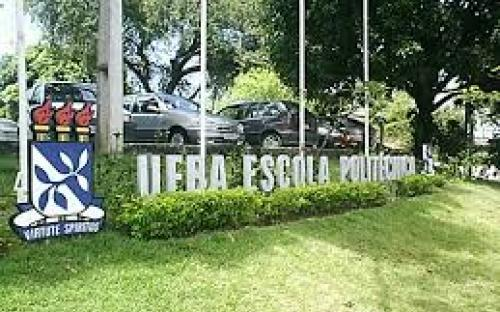
\includegraphics[width=0.29\textwidth]{biblioteca4_bernadeth}
    \end{wrapfigure}
    \subsubsection{Biblioteca Universitária Bernadeth Sinay Neves da Escola Politécnica}
        \begin{itemize}
            \item Horário de funcionamento: segunda a sexta-feira, das 8:00h às 22:00h e sábado, das 8:00h às 12:00h.
            \item Endereço: Rua Aristides Novis, n\textsuperscript{o} 2, Federação, 40210-630 - Salvador.
            \item Tel.: (71) 3283-9714/3283-9715/3283-9705
            \item E-mail: bieng@ufba.br
        \end{itemize}
        
        \begin{wrapfigure}{R}{0.3\textwidth}
            \centering
            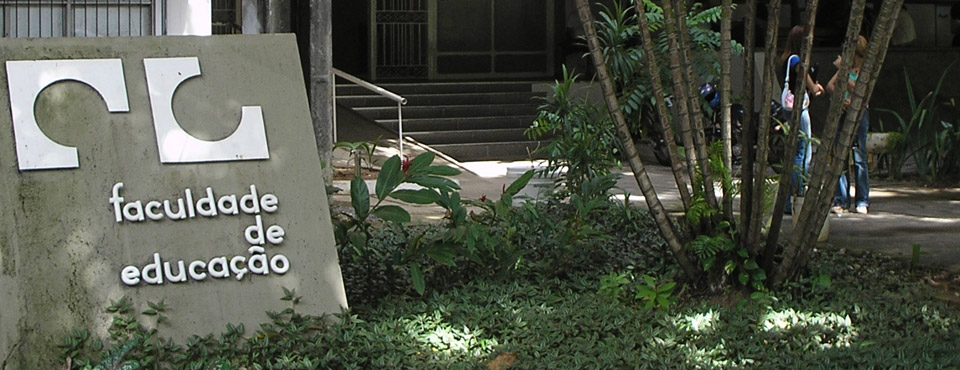
\includegraphics[width=0.29\textwidth]{biblioteca5_biedu}
        \end{wrapfigure}
    \subsubsection{Biblioteca Anísio Teixeira da Faculdade de Educação}
        \begin{itemize}
            \item Abriga acervo das áreas de Educação, Psicologia, Filosofia, Sociologia, Educação física, Esportes, Lazer.
            \item Endereço: Av. Reitor Miguel Calmon, s/n, Campus Universitário do Canela, 40110-100 - Salvador.
            \item Tel.: (71) 3283-7255/3283-7256
            \item E-mail: biedu@ufba.br
        \end{itemize}
        \newpage
        \begin{wrapfigure}{R}{0.3\textwidth}
            \centering
            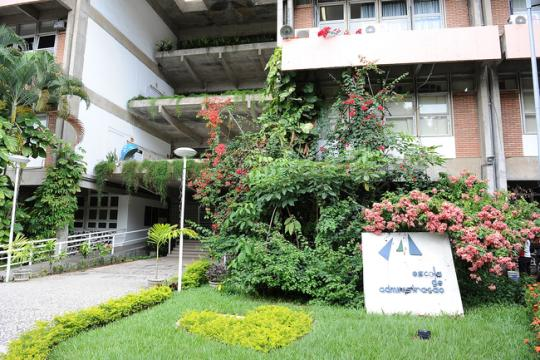
\includegraphics[width=0.29\textwidth]{biblioteca6_adm}
        \end{wrapfigure}
    \subsubsection{Biblioteca da Escola de Administração}
        \begin{itemize}
            \item Abriga acervo da Escola de Administração.
            \item Horário de funcionamento: segunda a sexta-feira, das 7:30h às 20:30h.
            \item Endereço: Av. Reitor Miguel Calmon, s/n, Campus Universitário do Canela, 40110-100 - Salvador.
            \item Tel.: (71) 3283-7636/3283-7337
            \item E-mail: dortas@ufba.br
        \end{itemize}
        \begin{wrapfigure}{R}{0.3\textwidth}
            \centering
            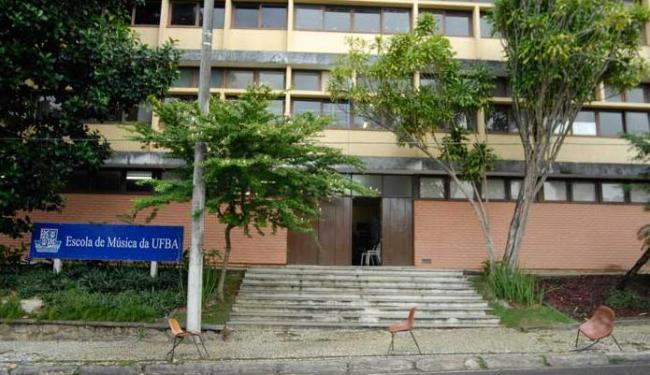
\includegraphics[width=0.29\textwidth]{biblioteca7_mus}
        \end{wrapfigure}
    \subsubsection{Biblioteca da Escola de Música}
        
        \begin{itemize}
            \item Abriga um acervo composto de livros, periódicos, partituras, discos de vinil, CDs e alguns DVDs.
            \item Horário de funcionamento: segunda a sexta-feira, das 7:00h às 19:00h.
            \item Endereço: Rua Basílio da Gama, s/n, Canela, 40160-060 - Salvador.
            \item Tel.: (71) 3283-7909/3283-7910
            \item E-mail: bibmus@ufba.br
        \end{itemize}
        \begin{wrapfigure}{R}{0.3\textwidth}
            \centering
            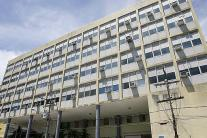
\includegraphics[width=0.29\textwidth]{biblioteca8_eco}
        \end{wrapfigure}
    \subsubsection{Biblioteca da Faculdade de Economia}
        \begin{itemize}
            \item Abriga acervo dos cursos de Ciências Econômicas.
            \item Horário de funcionamento: segunda a sexta-feira, das 7:00h às 19:00h.
            \item Endereço: Praça da Piedade, n\textsuperscript{o} 6, Centro, 40070-010 - Salvador.
            \item Tel.: (71) 3283-7587
            \item E-mail: fcebibl@ufba.br
        \end{itemize}
        \begin{wrapfigure}{R}{0.3\textwidth}
            \centering
            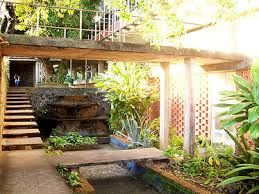
\includegraphics[width=0.29\textwidth]{biblioteca9_arq}
        \end{wrapfigure}
    
    \subsubsection{Biblioteca de Arquitetura}
        \begin{itemize}
            \item Abriga acervo dos cursos de Arquitetura e Urbanismo.
            \item Horário de funcionamento: segunda a sexta-feira, das 8:00h às 22:00h.
            \item Endereço: Rua Caetano Moura, n\textsuperscript{o} 121, Federação, 40210-350 – Salvador.
            \item Tel.: (71) 3283-5888
            \item E-mail: bibarq@ufba.br
        \end{itemize}
        \begin{wrapfigure}{R}{0.3\textwidth}
            \centering
            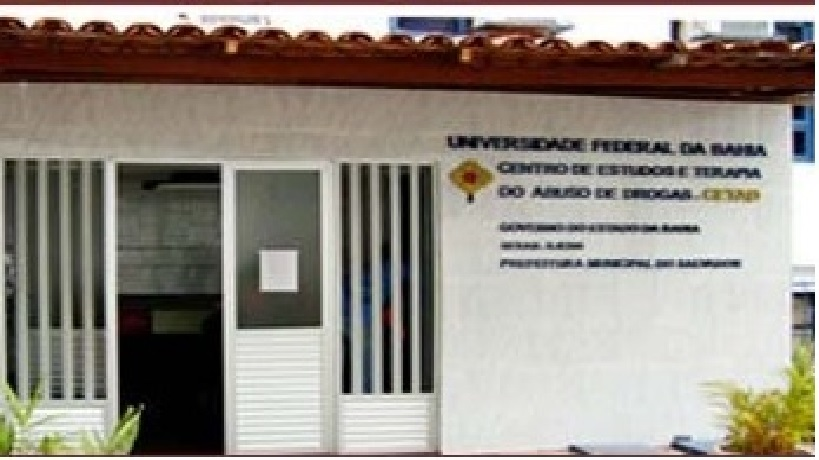
\includegraphics[width=0.29\textwidth]{biblioteca10_cetad}
        \end{wrapfigure}
    \subsubsection{Biblioteca do Centro de Estudos e Terapia do Abuso de Drogas – CETAD}
        \begin{itemize}
            \item Abriga acervo relacionado ao uso ou abuso de substâncias psicoativas.
            \item Horário de funcionamento: segunda a sexta-feira, das 8:00h às 12:00h e das 14:00h às 18:00h.
            \item Endereço: Rua Pedro Lessa, n\textsuperscript{o} 123 Canela, 40110-050 - Salvador.
            \item Tel.: (71) 3336-3322/3336-5341
            \item E-mail: bibliotecacetad@hotmail.com
        \end{itemize}
        \begin{wrapfigure}{R}{0.3\textwidth}
            \centering
            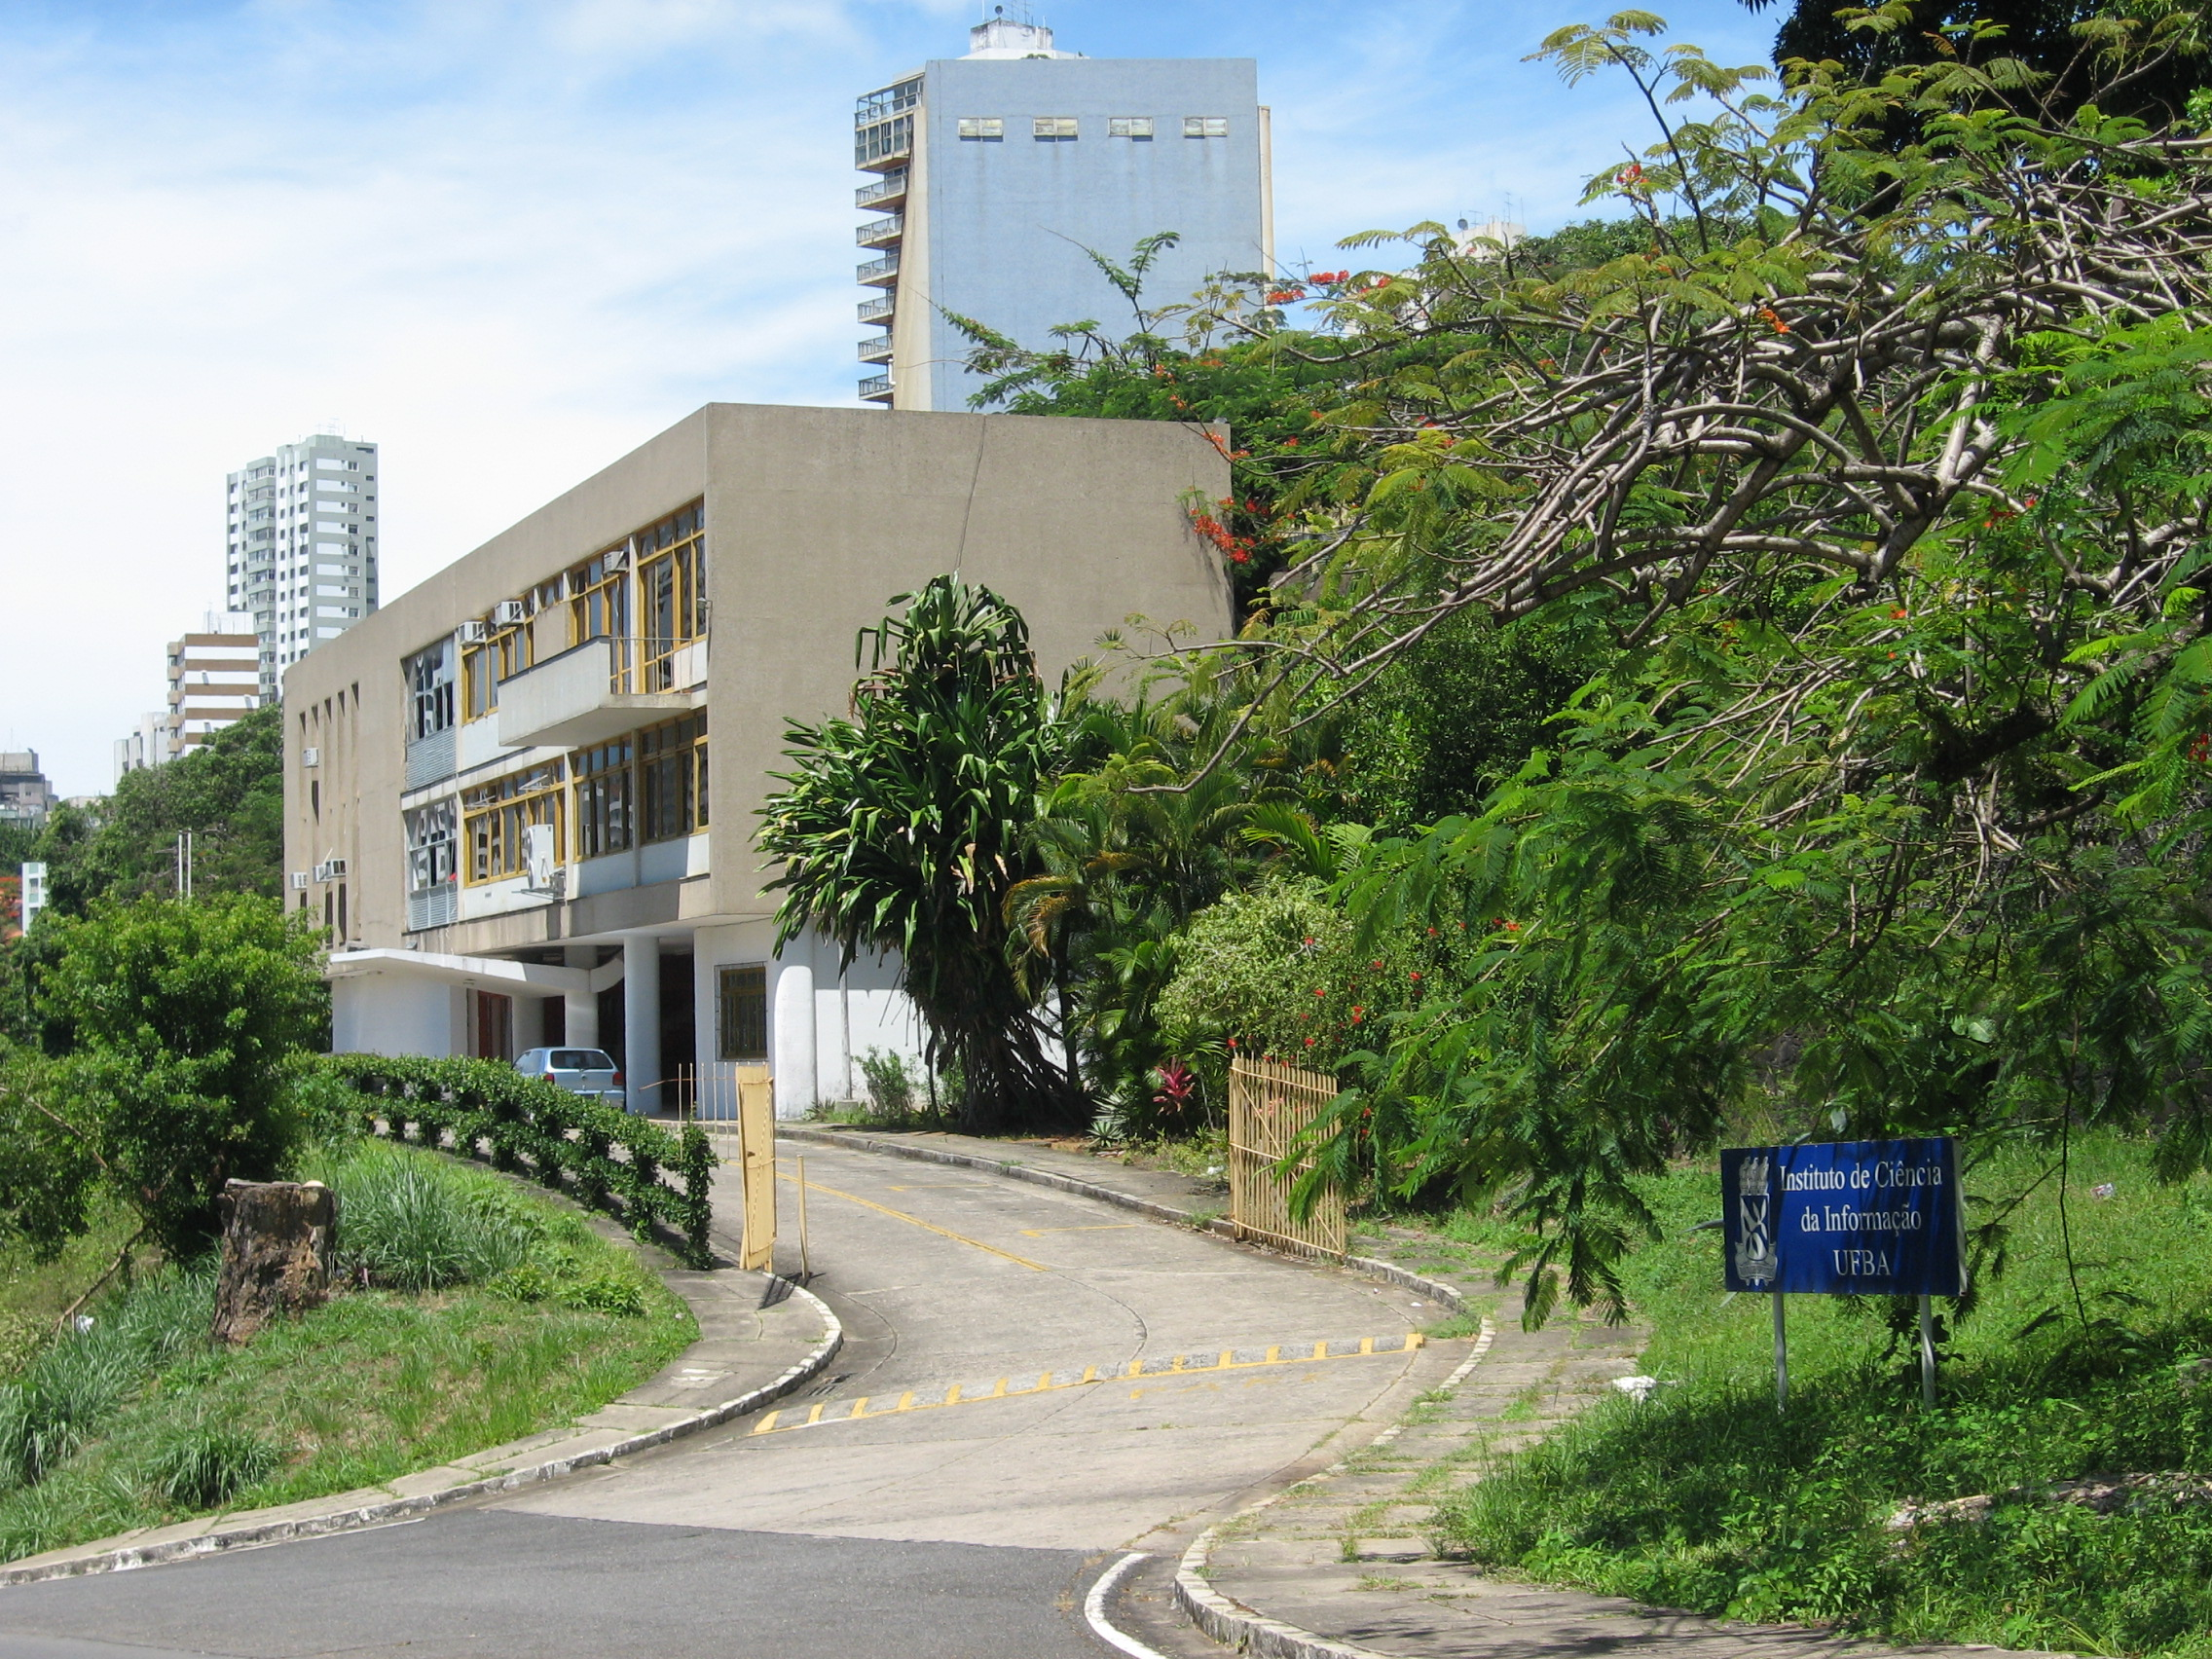
\includegraphics[width=0.29\textwidth]{biblioteca11_ici}
        \end{wrapfigure}
        \newpage
    \subsubsection{Biblioteca do Instituto de Ciência da Informação}
        \begin{itemize}
            \item Abriga acervo dos cursos de Ciência da Informação.
            \item Horário de funcionamento: segunda a sexta-feira, das 8:00h às 19:00h.
            \item Endereço: Av. Reitor Miguel Calmon, s/n, Canela, 40110-100 - Salvador.
            \item Tel.: (71) 3283-7757
            \item E-mail: bibici@ufba.br
        \end{itemize}
        \begin{wrapfigure}{R}{0.3\textwidth}
            \centering
            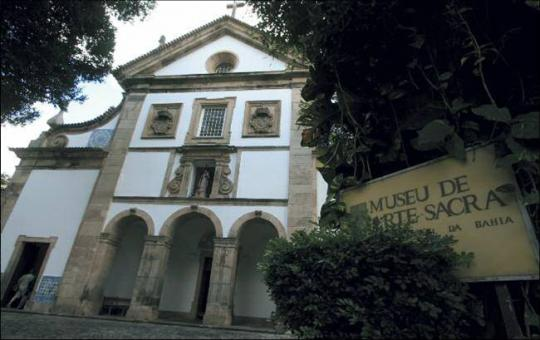
\includegraphics[width=0.29\textwidth]{biblioteca12_mas}
        \end{wrapfigure}
    \subsubsection{Biblioteca do Museu de Arte Sacra}
        \begin{itemize}
            \item Abriga acervo relativo a Religião, Arte, História, entre outros.
            \item Horário de funcionamento: segunda a sexta-feira, das 11:30h às 17:00h.
            \item Endereço: Rua do Sodré, n\textsuperscript{o} 276, Dois de Julho, 40060-240 - Salvador.
            \item Tel.: (71) 3283-5604
            \item E-mail: bibmas@ufba.br
        \end{itemize}
        \begin{wrapfigure}{R}{0.3\textwidth}
            \centering
            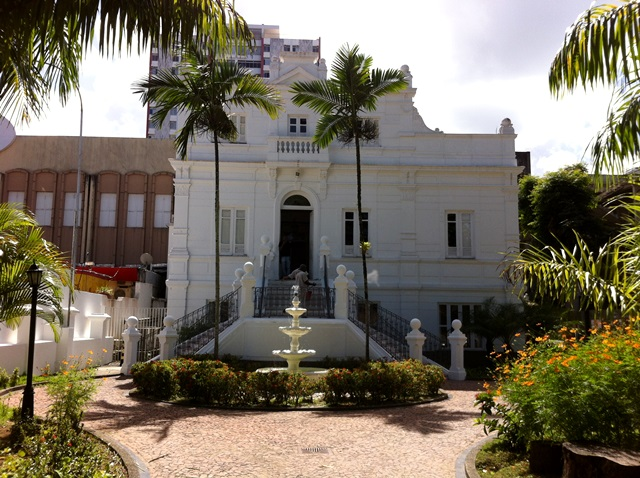
\includegraphics[width=0.29\textwidth]{biblioteca13_tea}
        \end{wrapfigure}
    \subsubsection{Biblioteca Nelson de Araújo da Escola de Teatro}
        \begin{itemize}
            \item Horário de funcionamento: segunda a sexta-feira, das 8:00h às 19:00h.
            \item Endereço: Rua Araújo Pinho, n\textsuperscript{o} 292, Canela, 40110-150 - Salvador.
            \item Tel.: (71) 3283-7873
            \item E-mail: bitea@ufba.br
        \end{itemize}
        \begin{wrapfigure}{R}{0.3\textwidth}
            \centering
            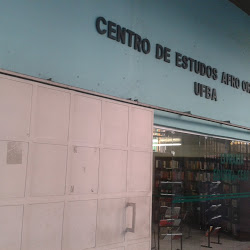
\includegraphics[width=0.29\textwidth]{biblioteca14_ceao}
        \end{wrapfigure}
   
    \subsubsection{Biblioteca do Centro de Estudo Afro-Oriental – CEAO}
        \begin{itemize}
            \item Horário de funcionamento: segunda a sexta-feira, das 8:00h às 19:00h.
            \item Endereço: Praça General Inocêncio Galvão, n\textsuperscript{o} 42, Largo 2 de Julho, 40060-055, Salvador.
            \item Tel.: (71) 3283-5515/3283-8628/3283-8630
            \item E-mail: biceao@ufba.br
        \end{itemize}
        \begin{wrapfigure}{R}{0.3\textwidth}
            \centering
            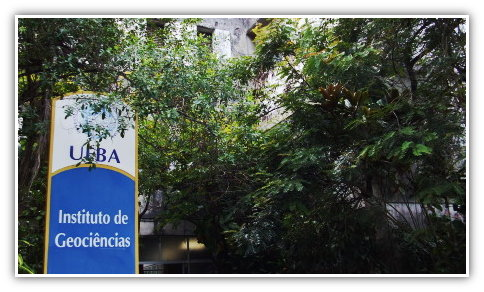
\includegraphics[width=0.29\textwidth]{biblioteca15_igeo}
        \end{wrapfigure}
    \subsubsection{Biblioteca Shiguemi Fujimori do Instituto de Geociências}
        \begin{itemize}
            \item Abriga acervo das áreas de Geografia, Geologia, Oceanografia e Geofísica.
            \item Horário de funcionamento: segunda a sexta-feira, das 8:00h às 21:00h.
            \item Endereço: Instituto de Geociências, Rua Barão de Jeremoabo, s/n, 3\textsuperscript{o} piso, Campus Universitário de Ondina, 40170-020 - Salvador.
            \item Tel.: (71) 3283-8628/3283-8630
            \item E-mail: bigeo@ufba.br
        \end{itemize}
        \newpage
        \begin{wrapfigure}{R}{0.3\textwidth}
            \centering
            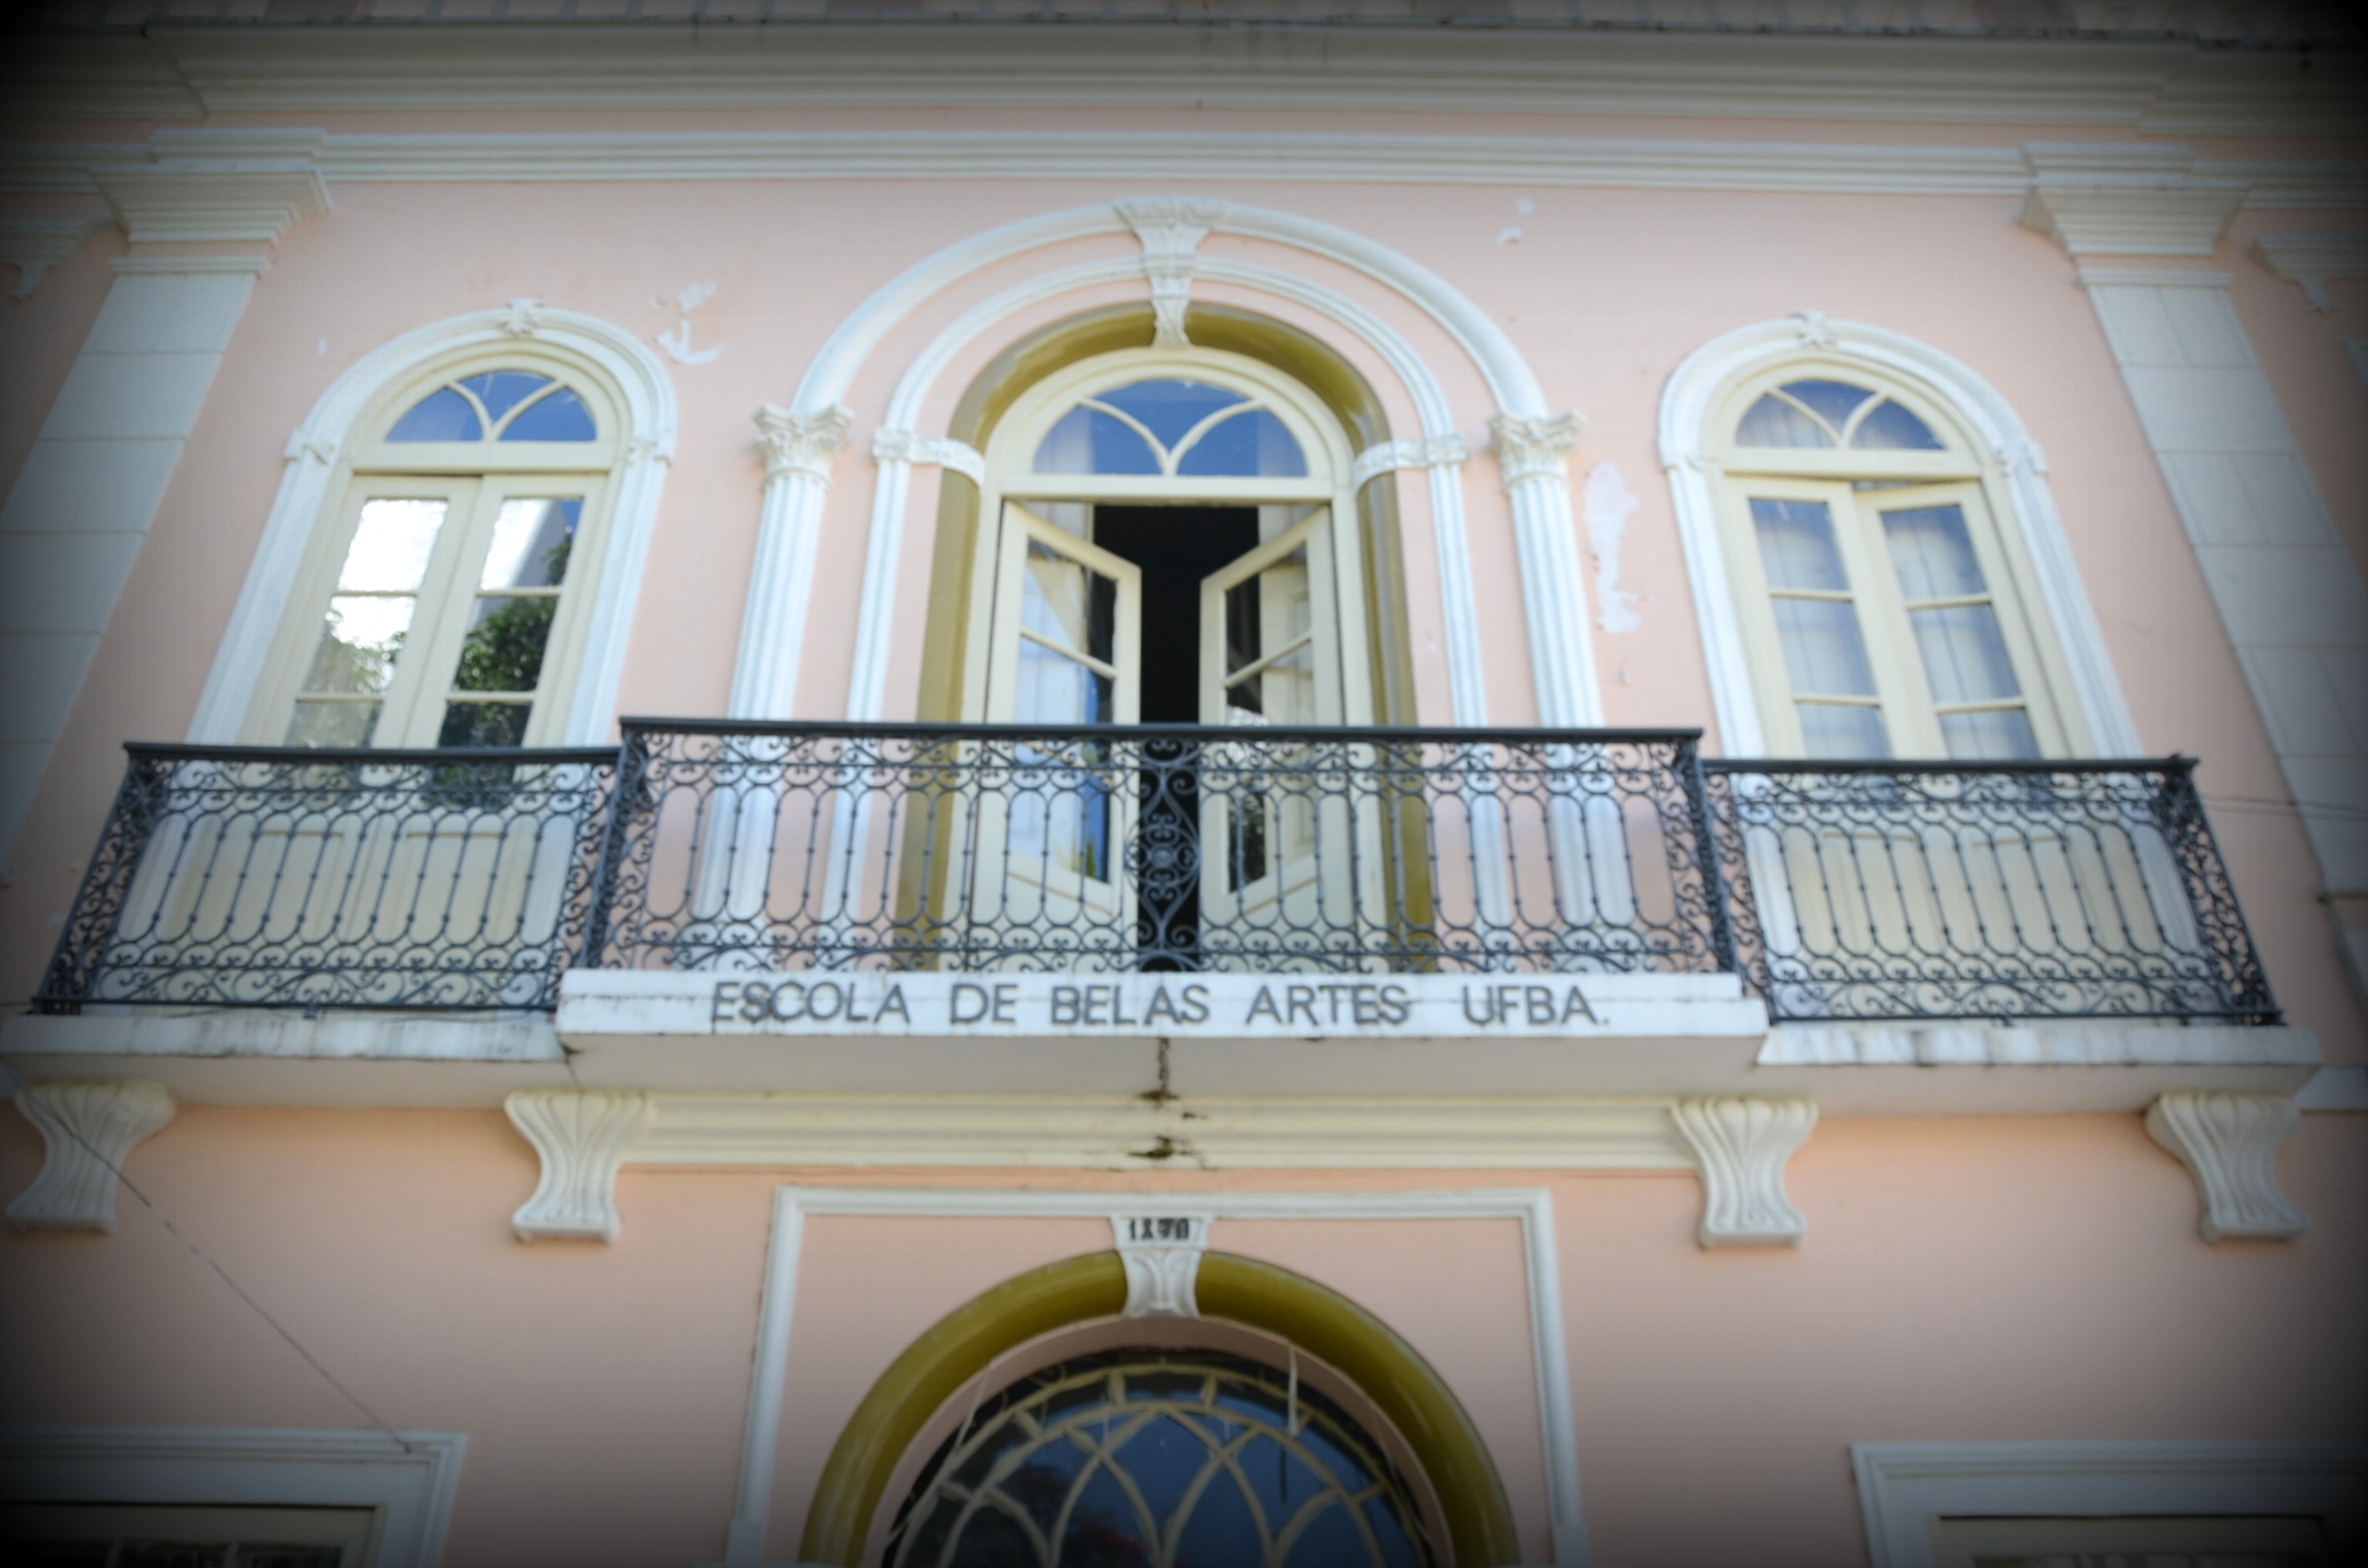
\includegraphics[width=0.29\textwidth]{biblioteca16_eba}
        \end{wrapfigure}
    \subsubsection{Biblioteca Sofia Olszewski Filha da Escola de Belas Artes}
        \begin{itemize}
            \item Horário de funcionamento: segunda a sexta-feira, das 8:00h às 19:00h.
            \item Endereço: Av. Araújo Pinho, n\textsuperscript{o} 212, Canela, 40110-150 - Salvador.
            \item Tel.: (71) 3283-7932
            \item E-mail: bibeba@ufba.br
        \end{itemize}
        \begin{wrapfigure}{R}{0.3\textwidth}
            \centering
            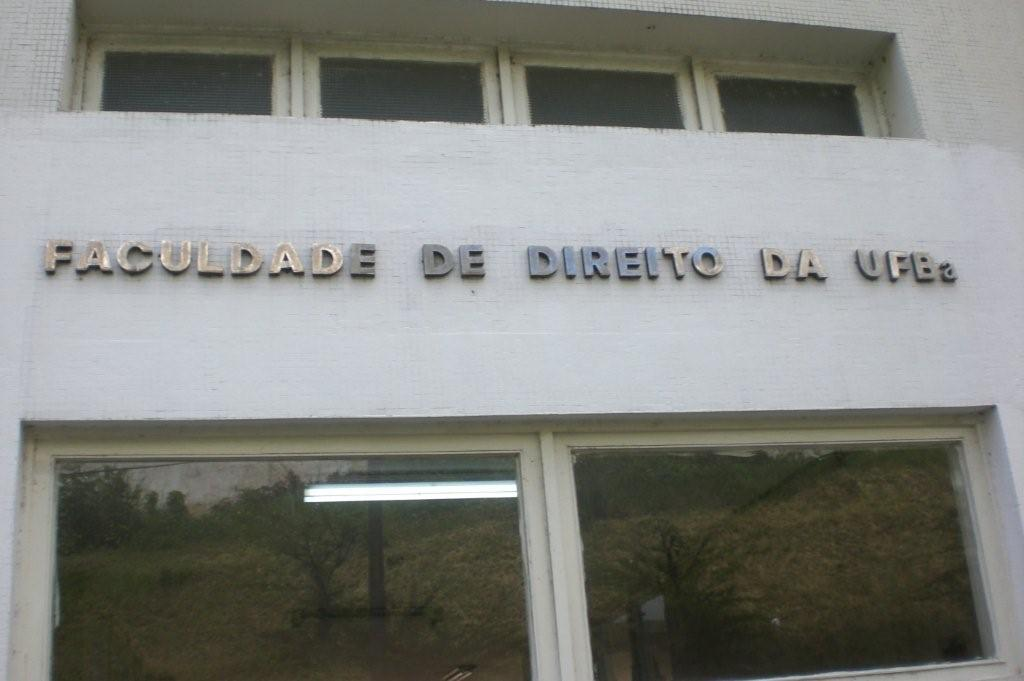
\includegraphics[width=0.29\textwidth]{biblioteca17_dir}
        \end{wrapfigure}
    \subsubsection{Biblioteca Teixeira de Freitas da Faculdade de Direito}
        \begin{itemize}
            \item Abriga acervo que abrange todas as áreas do direito.
            \item Horário de funcionamento: segunda a sexta-feira, das 8:00h às 22:00h e sábado das 8:00h às 13:00h.
            \item Endereço: Rua da Paz, s/n, 3\textsuperscript{o} andar, Graça, 40150-140 - Salvador.
            \item Tel.: (71) 3283-9059
            \item E-mail: bidir@ufba.br
        \end{itemize}
        \begin{wrapfigure}{R}{0.3\textwidth}
            \centering
            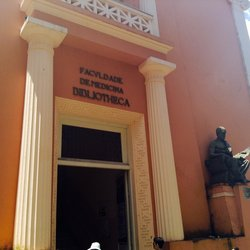
\includegraphics[width=0.29\textwidth]{biblioteca18_gon}
        \end{wrapfigure}
    \subsubsection{Biblioteca Professor Gonçalo Muniz e Memorial da Saúde Brasileira}
        \begin{itemize}
            \item Abriga extenso acervo das áreas de Medicina.
            \item Horário de funcionamento: segunda a sexta-feira, das 8:00h às 17:00h.
            \item Endereço: Largo Terreiro de Jesus Antiga Faculdade de Medicina, s/n, Pelourinho, 40026-010 - Salvador.
            \item Tel.: (71) 3283-5575
            \item E-mail: bibgm@ufba.br
        \end{itemize}
        \begin{wrapfigure}{R}{0.3\textwidth}
            \centering
            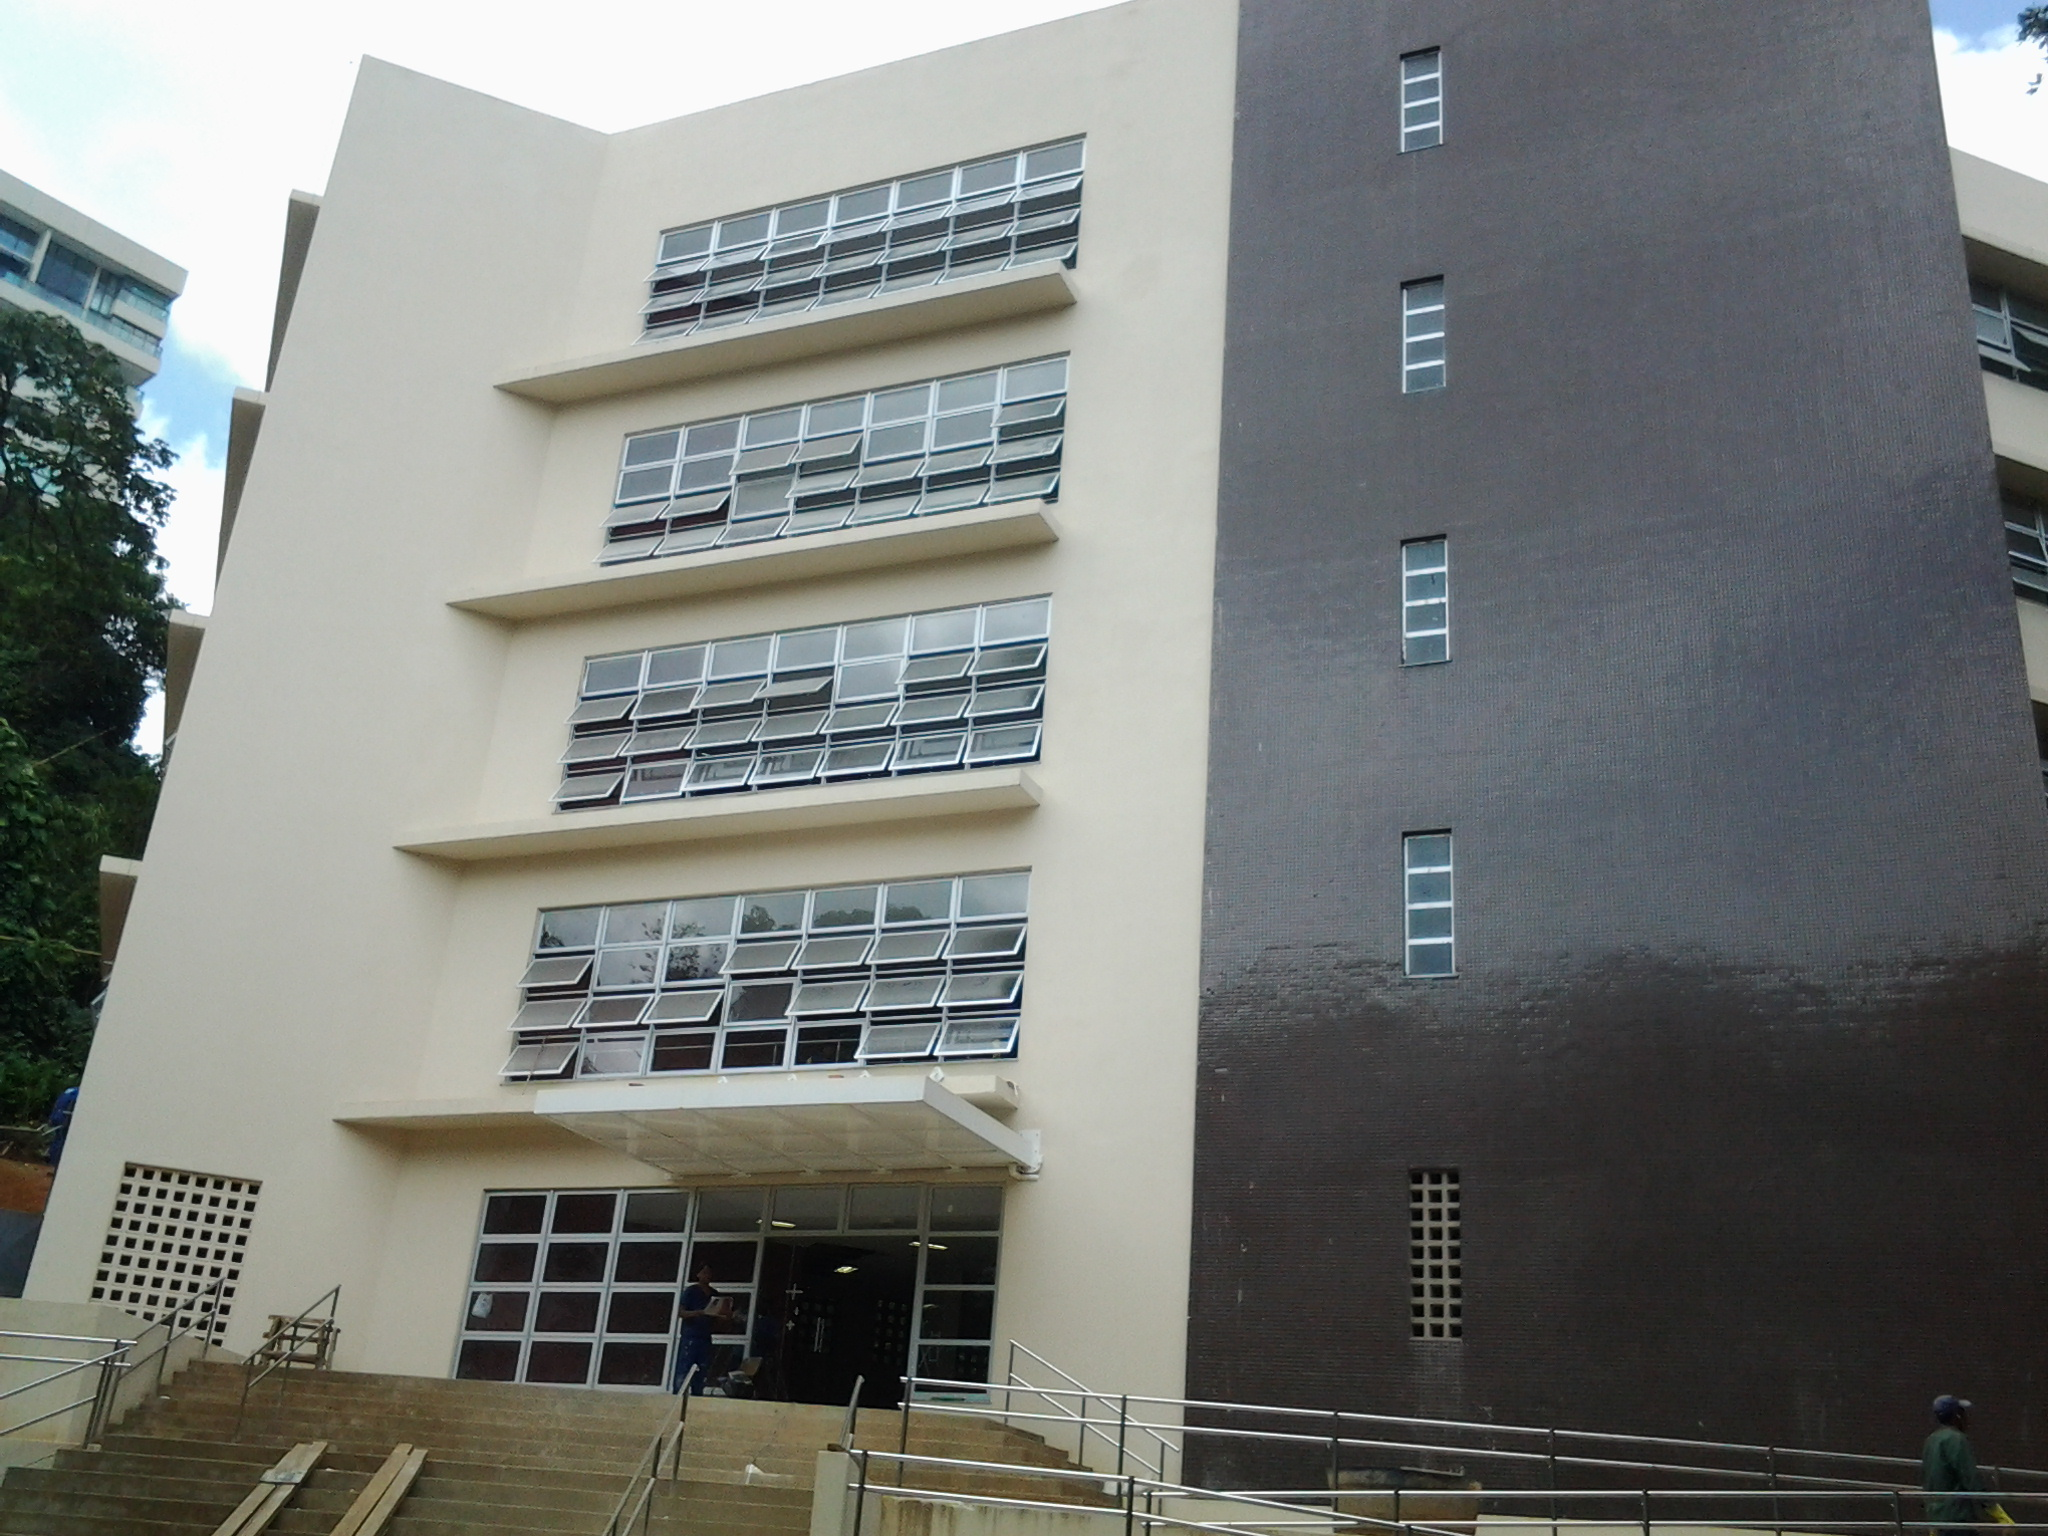
\includegraphics[width=0.29\textwidth]{biblioteca19_cont}
        \end{wrapfigure}
    \subsubsection{Biblioteca Prof. José Bernardo Cordeiro Filho - Faculdade de Ciências Contábeis}
        \begin{itemize}
            \item Abriga acervo dos cursos de Ciências Contábeis.
            \item Horário de funcionamento: segunda a sexta-feira, das 8:00h às 19:00h.
            \item Endereço: Avenida Reitor Miguel Calmon, s/n, Vale do Canela, 40110-903 – Salvador.
            \item Tel.: (71) 3283-8771
            \item E-mail: bibcontabeis@ufba.br
        \end{itemize}
        \begin{wrapfigure}{R}{0.3\textwidth}
            \centering
            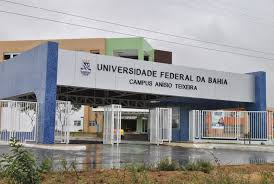
\includegraphics[width=0.29\textwidth]{ufba_cat}
        \end{wrapfigure}
    \subsubsection{Biblioteca do Campus Universitário Anísio Teixeira}
        \begin{itemize}
            \item Abriga acervo das áreas de atuação de cada curso do Campus.
            \item Horário de funcionamento: segunda a sexta-feira, das 7:00h às 19:00h.
            \item Endereço: Rua Rio de Contas, n\textsuperscript{o} 58, Candeias, 45029-094 - Vitória da Conquista.
            \item Tel.: (71) 3429-2721
            \item E-mail: bcat@ufba.br
        \end{itemize}
    \subsubsection{Consulta ao acervo, reserva e renovação}
        Através do sistema PERGAMUM os estudantes podem consultar o acervo bibliográfico das bibliotecas, bem como a quantidade disponível de exemplares. Os estudantes, por meio do número de matrícula e senha, podem também verificar o histórico de empréstimo, a data de devolução, fazer renovações e acompanhar as reservas.
        
        \begin{wrapfigure}{R}{0.3\textwidth}
            \centering
            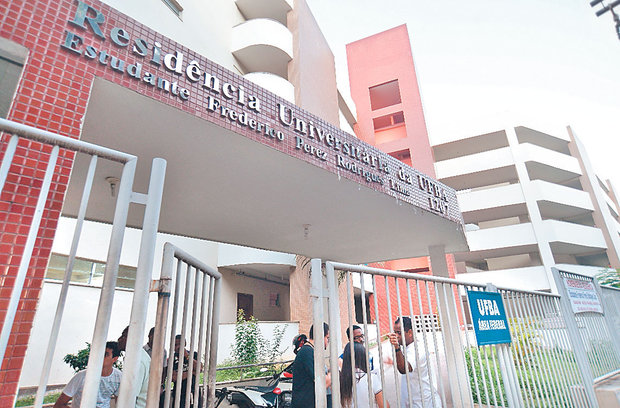
\includegraphics[width=0.29\textwidth]{residenciaUfba.jpg}
        \end{wrapfigure}
\section{Residências universitárias}
         Modalidade de acesso a moradia em que a UFBA, através de aparato próprio ou sob contrato, gerencia espaços onde são assegurados, além da moradia, áreas comuns para estudos e convivência, durante o tempo médio do curso.
         As Residências Universitárias da UFBA, em Salvador/Ba, são distribuídas em 4 complexos de moradias estrategicamente localizas próximas dos campi da Universidade. A 1ª localizada no Corredor da Vitória, a segunda no Largo da Vitória,a terceira na Graça e a quarta na Avenida Anita Garibaldi.
         
 
\section{Restaurantes universitários}
    \begin{wrapfigure}{L}{0.3\textwidth}
            \centering
            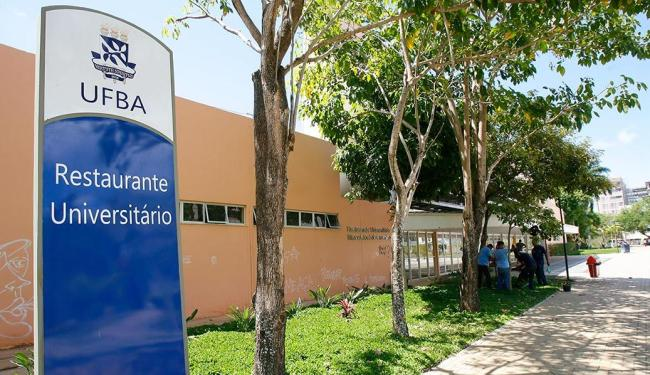
\includegraphics[width=0.29\textwidth]{RuUfba.jpg}
        \end{wrapfigure}
    O restaurante universitário da UFBA distribui refeições no período do almoço e da janta necessitando apenas apresentar o comprovante de matricula e pagar um valor de R\$ 2,50. Porém, as refeições são limitadas e distribuídas por ordem de chegada. Sendo o número de fichas em torno de 400, é preciso chegar com certa antecedência para conseguir pegar a refeição. São oferecidas duas opções: vegetariana e tradicional.

%desconfigurou
\section{Creche}
    \subsubsection{Auxílio Creche}
        Estudantes em vulnerabilidade socioeconômica têm o direito ao Auxílio Creche que consiste em um auxílio para custeio de despesas com cuidado e serviço de educação infantil na faixa etária de 4 (quatro) meses a 3 (três) anos e 11 (onze) meses de idade.
        Os estudantes devem estar regulamente matriculados em curso de graduação e não podem ter vínculo empregatício.
        \begin{wrapfigure}{R}{0.3\textwidth}
            \centering
            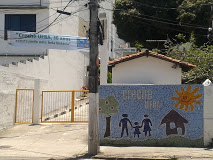
\includegraphics[width=0.29\textwidth]{creche}
        \end{wrapfigure}
    \subsubsection{Serviço Creche UFBA}
        A Creche UFBA é uma unidade vinculada à PROAE que atende crianças filhas de estudantes, servidores e professores da UFBA, com idades entre 4 (quatro) meses a 3 (três) anos e 11 (onze) meses. Constitui-se de um espaço de aprendizado que promove atividades educativas e culturais, contribuindo para o desenvolvimento educacional e psicológico da criança.
        A depender da idade*, as crianças são divididas nos seguintes grupos:
            \begin{itemize}
                \item Berçário - 4 meses
                \item Grupo 1 - 1 ano
                \item Grupo 2 - 2 anos
                \item Grupo 3 - 3 anos
            \end{itemize}
            \begin{remark}
                * Idade da criança até março do ano atual
            \end{remark}
        A comunicação entre a Creche UFBA e os pais é feita através de reuniões gerais, reuniões individualizadas (ou por pequenos grupos) e pela comissão de pais.
    \subsubsection{Horários de atendimento da Creche UFBA}
        Os horários da Creche UFBA obedecem ao calendário acadêmico e seu funcionamento ocorre de segunda a sexta-feira (exceto em feriados e pontos facultativos) e possui dois regimes:
        \begin{itemize}
            \item integral - das 7 às 18 horas
            \item parcial - das 7 às 13 horas no turno matutino ou das 13 às 18 horas no turno vespertino
        \end{itemize}

\section{Serviço Médico Universitário Rubens Brasil}
    \begin{wrapfigure}{R}{0.3\textwidth}
            \centering
            
\includegraphics[width=0.29\textwidth]{smurb.jpg}
        \end{wrapfigure}         
        O SMURB – Serviço Médico Universitário Rubens Brasil – foi criado em 1952 para atender os estudantes carentes, mas com a entrada do Doutor Rubens Brasil o serviço foi ampliado para os docentes, funcionários e seus respectivos familiares. Para ter acesso a este serviço o associado a UFBA tem de passar por uma triagem que é requisitada no momento de ingresso na universidade.

\section{BUZUFBA}
\begin{wrapfigure}{L}{0.3\textwidth}
	\centering
	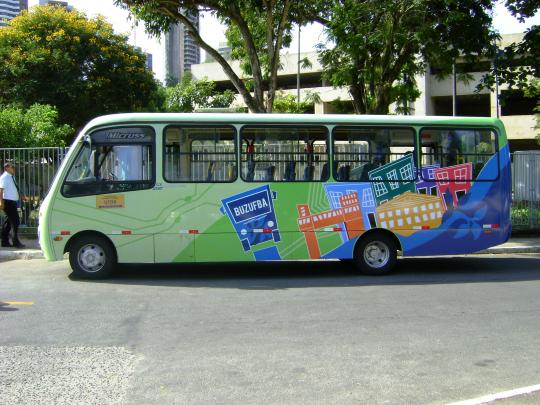
\includegraphics[width=0.29\textwidth]{buzufba}
\end{wrapfigure}
Os estudantes da UFBA podem contar com o serviço gratuito dos BUZUFBAS. 
A frota conta com cinco BUZUFBAS, dois que foram recentemente adicionados.

    O BUZUFBA é o sistema de transporte intercampi da UFBA conquistado após a greve de 2012. É um serviço gratuito planejado para facilitar a locomoção dos estudantes que têm aulas nos diversos campi da UFBA em Salvador, visando diminuir o tempo de locomoção entre um campus e outro, além de evitar gastos com o transporte público podendo ser utilizado pela comunidade. 
    
    As variadas rotas perpassam os distribuídos campi com horários fixos. O serviço é bastante útil mas precisa ser melhorado em relação ao tamanho da frota e aos horários de modo que não haja superlotação.

\section{Bolsas e auxílios}
    \subsubsection{Auxílios financeiros}
        Alunos em vulnerabilidade socioeconômica, regulamente matriculados em curso de graduação da UFBA e que não possuam vínculo empregatício têm direito a vários auxílios financeiros.
    \subsubsection{Auxílio Moradia}
        Auxílio mensal destinado ao custeio de parte das despesas com moradia até a conclusão da primeira graduação. Os estudantes também terão garantidas duas refeições diárias no Restaurante Universitário e a opção de complementação financeira para custear até mais duas refeições diárias.
    \subsubsection{Auxílio Transporte}
        Auxílio mensal referente ao valor de 3 (três) meias-passagens de ônibus para seis dias semanais destinado ao custeio das despesas de deslocamento.
    \subsubsection{Auxílio a Pessoa com Necessidades Educativas Especiais}
        Auxílio mensal destinado à estudantes de graduação que apresentem deficiência física, intelectual ou sensorial (auditiva ou visual), transtornos globais do desenvolvimento e altas habilidades e superdotação.  Os estudantes também terão a opção de complementação financeira para custear até duas refeições diárias.
    \subsubsection{Serviço de Alimentação}
        Garantia de duas refeições diárias realizadas no Restaurante Universitário.
\begin{wrapfigure}{R}{0.3\textwidth}
    \centering
    
\includegraphics[width=0.29\textwidth]{permanecer}
\end{wrapfigure}
\subsection{Programa Permanecer}
        Destinado a estudantes em vulnerabilidade socioeconômica na universidade, visando assegurar a permanência bem-sucedida e garantindo a terminalidade dos estudos em nível de graduação.Para participar, o aluno deve submeter de projetos, para avaliação, em uma das áreas de Iniciação: Extensão,Ensino, Pesquisa ou Aprendizagens Profissionais. 